\begin{frame}{Scientific Method: A Common Misconception}
	\textbf{Science is not a linear process.}

	The common Scientific method is an
	oversimplification.

	\begin{figure}
		\centering
		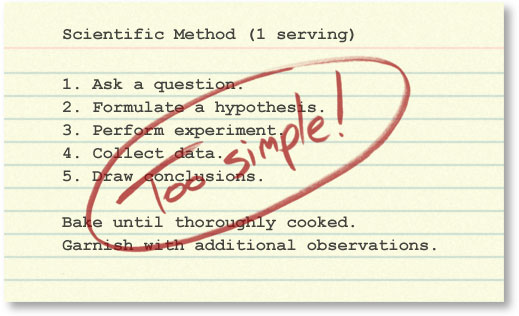
\includegraphics[width=0.7\textwidth]{Figures/sciencerecipe.jpg}
		\caption{The myth of the step-by-step "science recipe". \cite{Science}}
	\end{figure}

\end{frame}

\begin{frame}{How Does Science Actually Work?}
	\begin{columns}

		\column{0.6\textwidth}
		\textbf{Science operates through an iterative, interconnected process:}

		\vspace{0.3cm}
		\begin{itemize}
			\item \textbf{Observation} – Collecting empirical data from experiments or nature.
			\item \textbf{Hypothesis Testing} – Formulating and systematically evaluating explanations.
			\item \textbf{Peer Feedback} – Refining theories through collaboration and critique.
			\item \textbf{Application} – Translating scientific knowledge into real-world innovations.
		\end{itemize}

		\column{0.4\textwidth}
		\begin{figure}
			\centering
			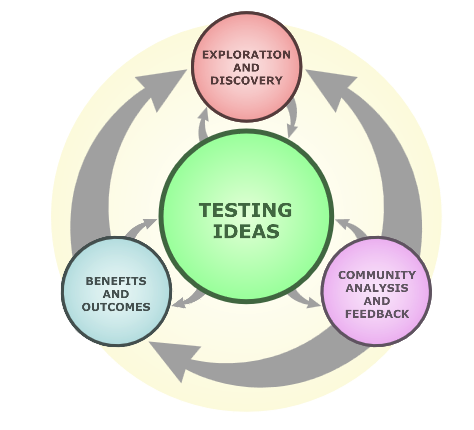
\includegraphics[width=\textwidth]{Figures/canvas.png}
			\caption{Science as a dynamic, self-correcting process. \cite{Science}}
		\end{figure}

	\end{columns}
\end{frame}

\begin{frame}{The Core of Science: Testing Ideas}
	\textbf{Empirical testing is the foundation of science.}

	Through experimentation and analysis, hypotheses are refined, rejected, or strengthened.
	\vspace{-0.2cm}
	\begin{figure}
		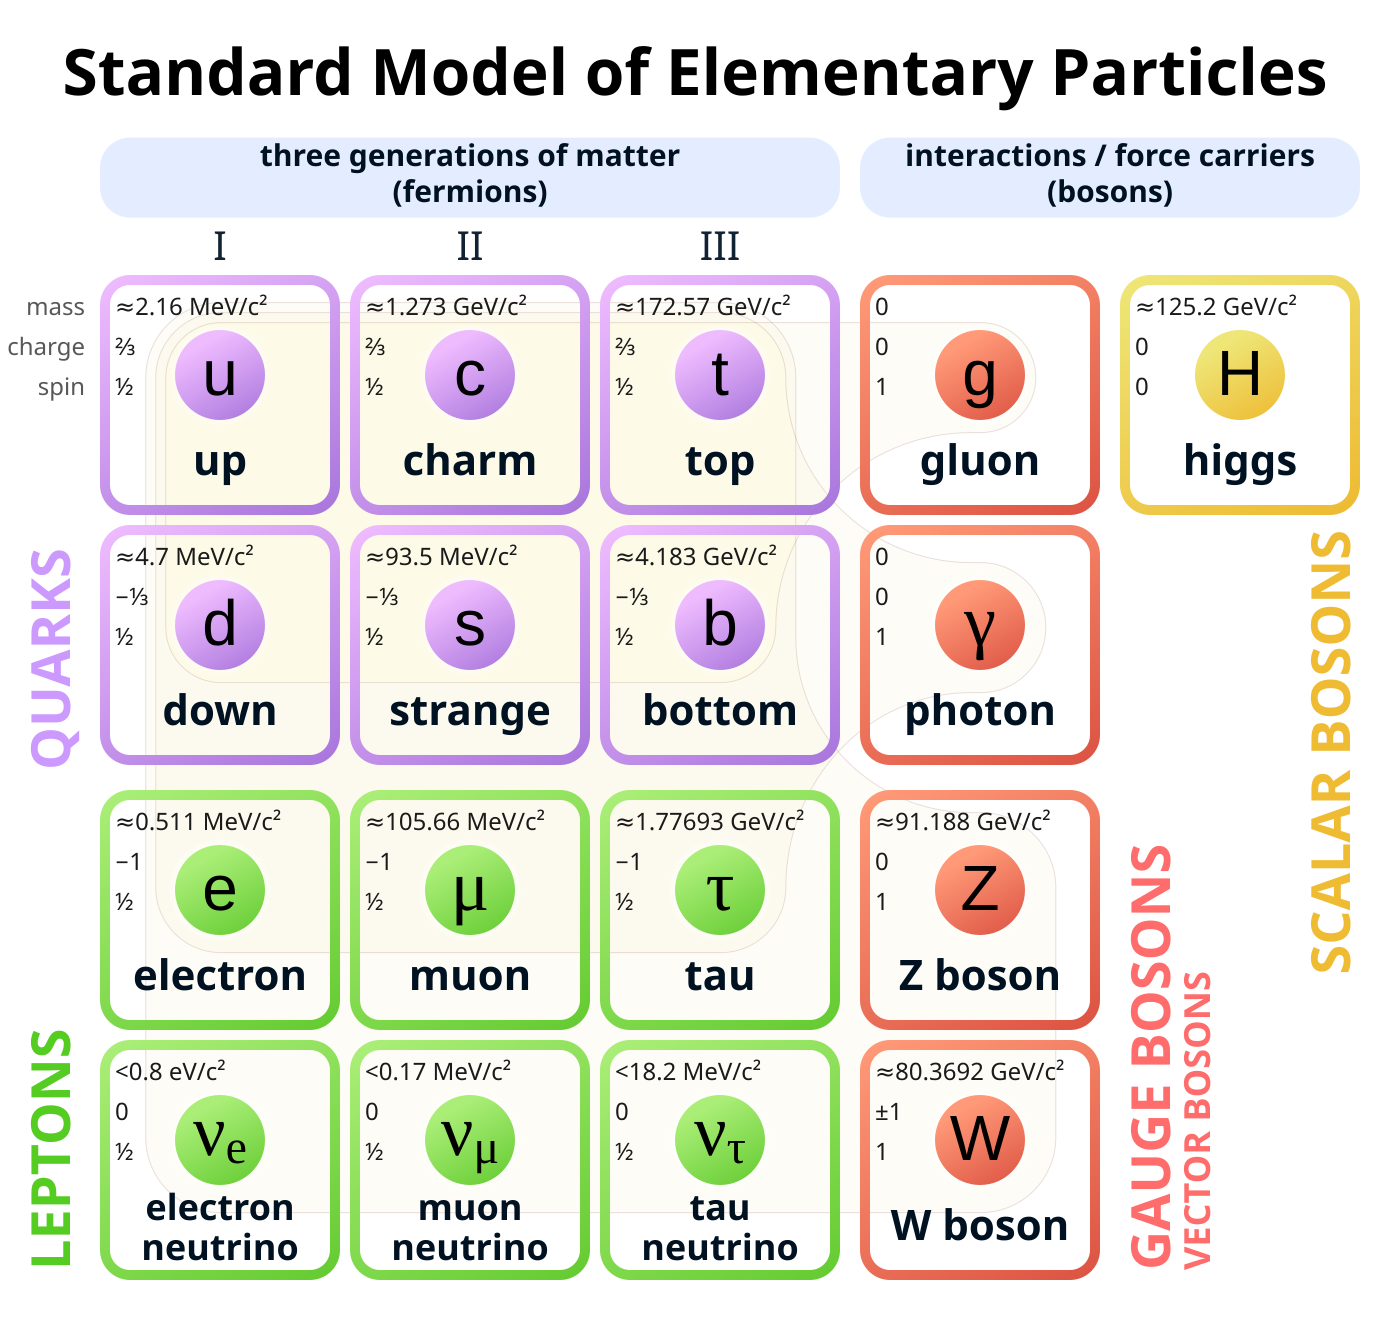
\includegraphics[width=0.5\textwidth]{Figures/Standard-Model.png}
		\vspace{-0.5cm}
		\caption{The Standard Model: A theory refined through decades of testing. \cite{Cush2019}}
	\end{figure}

\end{frame}
